\documentclass[10pt,landscape]{beamer}
\usepackage[latin1]{inputenc}
\usepackage{amsmath}
\usepackage{amsfonts}
\usepackage{amssymb}
\title{SteriaQuiz}
\usepackage{xcolor}
\definecolor{SteriaOrange}{rgb}{1.,0.72.,0.}
\definecolor{SteriaBlue}{rgb}{0.016,0.192,0.357} 
\begin{document}
	\setbeamercolor{background canvas}{bg=SteriaOrange}

	\setbeamercolor{frametitle}{fg=SteriaBlue}
	\setbeamercolor{item projected}{fg=SteriaBlue}
	\begin{frame}
		\begin{center}
		\textcolor{SteriaOrange}{.\\.\\}
			\textcolor{SteriaBlue}{{\Huge \textbf{SteriaQuiz}}{\Large\\JavaZone-profileringsgruppa}}
			
		\end{center}
	\end{frame}
	\begin{frame}{Hva gikk oppgaven ut p�?}
		\begin{itemize}
			\item[] Lage en konkurranse med en legorobot
			\item[] Lage en Steria-quiz 
		\end{itemize}
	\end{frame}

	\begin{frame}{Hva har vi gjort?}
		\begin{itemize}
			\item[] Bygget lego
			\item[] Laget quiz
			\item[] (som vi skal presentere snart)
			\item[] Drukket kaffe
		\end{itemize}
	\end{frame}
	
	{\usebackgroundtemplate{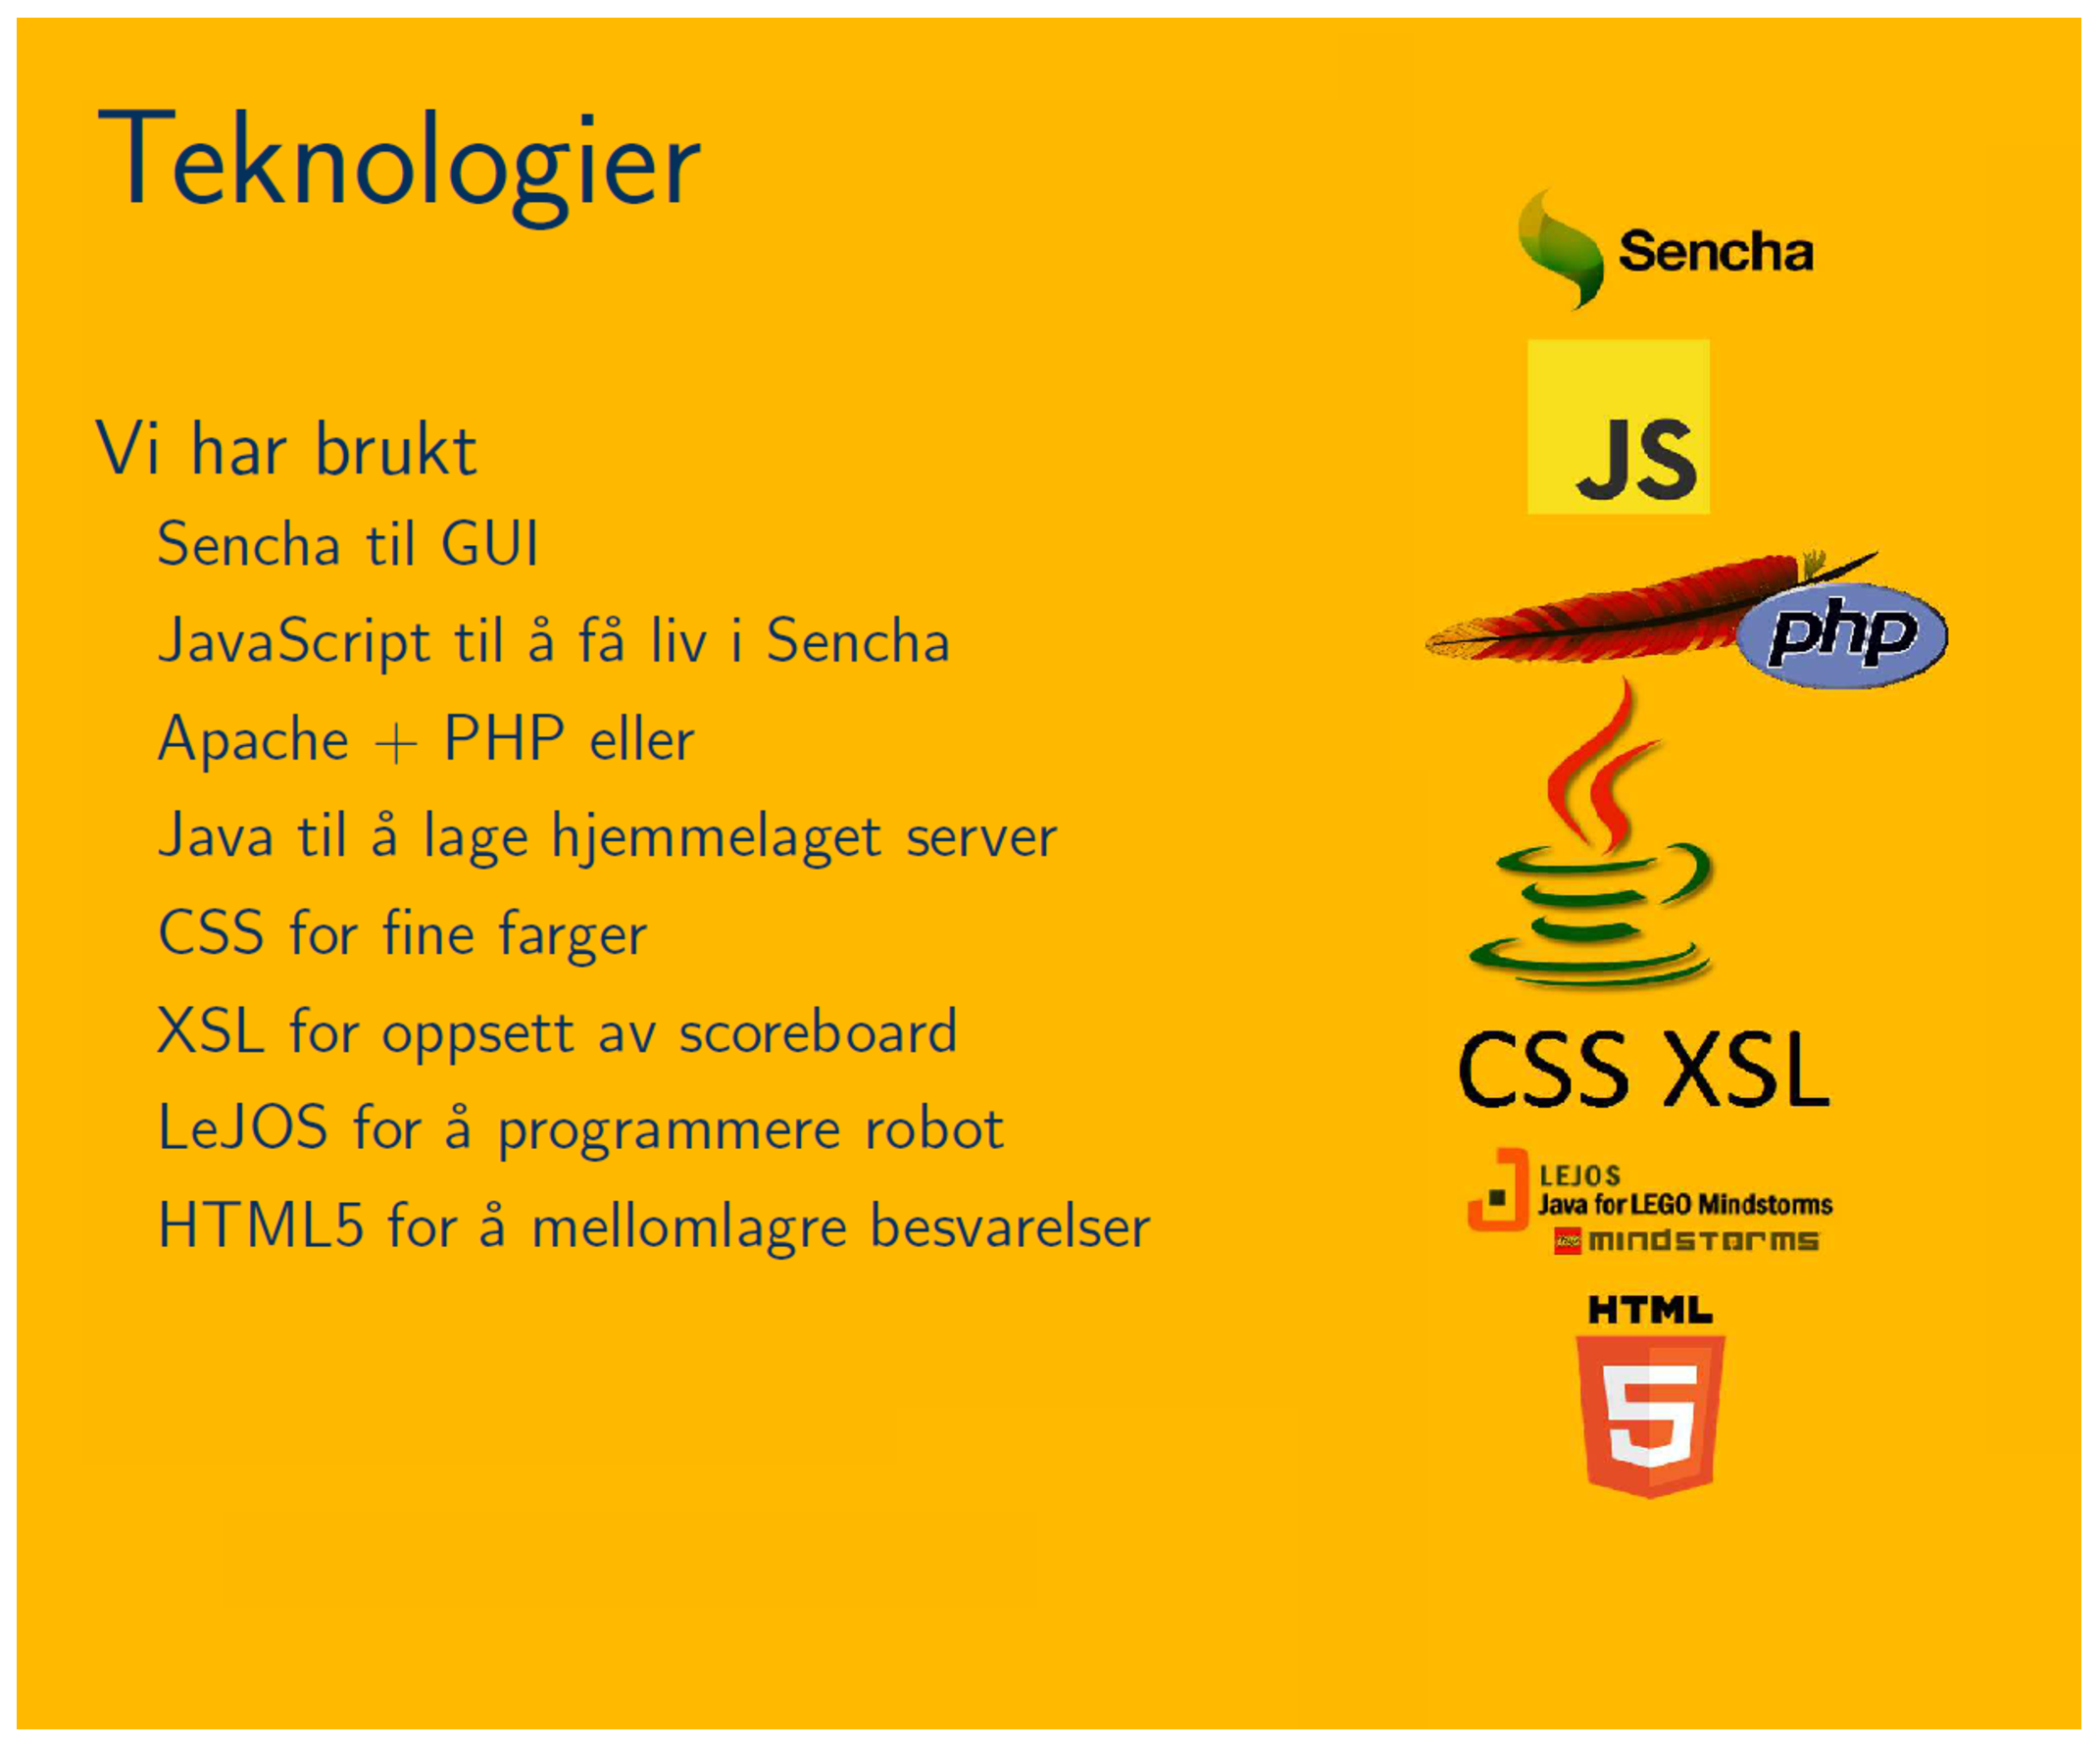
\includegraphics[width=\paperwidth]{Logop.eps}}
	\begin{frame}{}
	\end{frame}
	}
	
	\begin{frame}{Hva har vi ikke gjort?}
		\begin{itemize}
			\item[] testet nok
			\item[] testet mange nok forskjellige enheter
		\end{itemize}
		...men vi er rimelig sikre p� at det funker i en del tilfeller
	\end{frame}
	

	{\usebackgroundtemplate{
\includegraphics[height=\paperheight]{qr.eps}}
	\begin{frame}{}
	\end{frame}
	}
\end{document}